\documentclass{report}
\usepackage[utf8]{inputenc}
\usepackage{graphicx}
\usepackage{multirow}
\usepackage{caption}
\usepackage{subcaption}
\usepackage{amsfonts}
\usepackage[utf8]{inputenc}
\usepackage[spanish]{babel}
\usepackage{lscape}
\usepackage[left=1.5cm,right=1.5cm,top=2cm,bottom=2cm]{geometry}

\begin{document}

\begin{center}
    
    \begin{tabular}{l c r}
    
\includegraphics[scale=0.15]{Imagenes/IPN.jpeg}
    & 
        \bf\fontsize{22}{0}{\selectfont{Instituto Polit\'ecnico Nacional}}

    
    & 
\includegraphics[scale=0.08]{Imagenes/escom.png} \\
     
    & \bf\fontsize{22}{0}{\selectfont{ Escuela Superior de C\'omputo}} &  \\
    \end{tabular}

	
	\vspace*{2\baselineskip}
	
	{
		\bf\fontsize{12}{0}{\selectfont{An\'alisis de Algoritmos, Sem: 2021-1, 3CV1, Pr\'actica 1, 19/10/20}}
	}
			
	\vspace*{2\baselineskip}
			 
	{
		\fontsize{23}{0}{\selectfont{Práctica 1: Determinación Experimental de la Complejidad Temporal de un Algoritmo}}
	}
	
	\vspace*{2\baselineskip}
	
	{
		\bf\fontsize{12}{0}{\selectfont{Valle Mart\'inez Luis Eduardo, Rivero Ronquillo Omar Imanol}}
	}
	
	\vspace*{1\baselineskip}
	
	{
		\fontsize{12}{0}{\textit{lvalle212@gmail.com, imanol.rivero7@gmail.com}}
	}
	
	\vspace*{2\baselineskip}

    {
	    \fontsize{12}{0}\selectfont{
	    \textbf{Resumen:} En esta práctica fueron desarrollados dos algoritmos, para calcular la complejidad temporal de los mismos utilizando los ejemplos vistos en clase.}
	    
	    \fontsize{12}{0}\selectfont{
	    \textbf{Palabras Clave:} Complejidad, Algoritmos, Java.}
	
	}
\end{center}

\section*{Introducción} 
    En matem\'aticas, ciencias de la computaci\'on y disciplinas relacionadas, un algoritmo es un conjunto de instrucciones o reglas bien definidas, ordenadas y finitas que permite realizar una actividad mediante pasos sucesivos. Un algoritmo se compone de tres partes: Entrada, salida y proceso, siendo el proceso la serie de los pasos ejecutados. La importancia de los algoritmos en nuestra vida moderna es invaluable, pues las grandes comodidades de las que gozamos todos los dias tienen involucrados algoritmos simples o complejos.\par
    
    Por lo general existen una variedad de algoritmos para resolver el mismo problema, por lo que es necesario determinar cual es el mejor entre todos, esto solamente es posible de saber cuando de realiza un análisis obteniendo la complejidad del algoritmo.\par
    
    La finalidad de esta práctica es la de determinar la complejidad temporal de los algoritmos propuestos, generando gráficas que reflejen los resultados obtenidos.
    
\section*{Conceptos B\'asicos}
    Para comprender el trabajo realizado en esta práctica debemos revisar algunos conceptos.
    \begin{itemize}
        \item\textbf{Notaci\'on Big $\theta$:} Si $f(n)\in \theta (g(n))$, entonces $f(n)\geq 0$ $\forall n\in$ $\mathbb{N}$, tales funciones son llamadas asint\'oticamente no negativas o asint\'oticamente positivas.Cuando usamos la notaci\'on big $\theta$, estamos diciendo que una cota asint\'oticamente ajustada sobre el tiempo de ejecuci\'on. Es "asint\'oticamente" porque importa \'unicamente para los valores grandes de $n$. 
        \item\textbf{Notaci\'on Big $O$}: Dado una funci\'on $g(n),\mathbb{O}(g(n))$ denota el conjunto de funciones como: $\mathbb{O}(g(n) =\{f(n):\exists n$ $ C>0$ y $n_0>0$ tal que $0\le f(n) \le cg(n)$ $\forall n \geq n_0\}$. Usamos la notaci\'on O grande para las cotas superiores asint\'oticas, ya que acota el crecimiento del tiempo de ejecución por arriba para entradas suficientemente grandes.
        \item\textbf{Notaci\'on Big $\Omega$:} Dadas dos funciones $f(n)$ y $g(n), f(n)\in O(g(n))$ si $f(n)\in \Omega(g(n))$. Usamos la notaci\'on $\Omega$ grande para l\'imites asint\'oticos inferiores, ya que acota el crecimiento del tiempo de ejecuci\'on por abajo para entradas de tamaños suficientemente grandes.
    \end{itemize}
    
    \subsection*{Suma binaria}
         La implementación del algoritmo utilizado para sumar arreglos de 2 números binarios, se basó en un \textit{medio sumador}, que es un circuito común y sencillo en el ámbito de la electrónica digital.
                
                \hfill \break
        
                Se considera:\\
                \textbf{r}: Número potencia de 2\\
                \textbf{A}: Arreglo de tamaño \textbf{r}, cada índice contiene 1 bit(\textit{1},\textit{0}) representando un número binario donde: $0\leq$ \textbf{Binario} $\leq 2^r -1$\\
                \textbf{B}: Arreglo de tamaño \textbf{r}, cada índice contiene 1 bit(\textit{1},\textit{0}) representando un número binario donde: $0\leq$ \textbf{Binario} $\leq 2^r -1$\\
                \textbf{C}: Arreglo de tamaño \textbf{r+1}, almacena el resultado de la suma binaria en \textbf{A} y \textbf{B}.
                
                \hfill \break
                
                Tomándolo como un \textit{medio sumador} con 2 números de 1 bit, se guarda en un arreglo \textit{C}, el valor de la operación \textbf{XOR} de A[i], B[i] y el acarreo. Se guarda el acarreo resultado de esos 2 bits y mediante un \textit{for}, se avanza de forma descendente en los arreglos A y B. \\
                
                Pseudoc\'odigo:\\
            
                \begin{verbatim}
                * Notación
                    ^ = XOR
                    | = OR
                    & = AND
                
                    SumaBinaria(A,B,r)
                        acarreo = 0
                        for i=r-1  to i>=0 do
                            C[i+1] = acarreo ^ A[i] ^ B[i];
                            acarreo = (acarreo & A[i]) | (acarreo & B[i]) | 
                            (A[i] & B[i])
                        C[0] = (acarreo > 0) ? 1 : 0
                        return C
                \end{verbatim}
                
    \subsection*{Algoritmo de Euclides(MCD)}
        El algoritmo de Euclides es una t\'ecnica para encontrar r\'apidamente el M\'aximo Com\'un Divisor(MCD) entre 2 números enteros.\\
                
                El procedimiento encontrará el MCD cuando el residuo de la división es igual a 0. Los pasos a realizar son los siguientes:
                
                \begin{enumerate}
                    \item Se divide el número mayor entre el menor
                    \item Si el residuo no es igual a 0 el divisor será el MCD. En caso contrario se sigue el siguiente paso
                    \item Se divide ahora el divisor entre el residuo. Se siguen estos pasos hasta encontrar un residuo igual a 0
                \end{enumerate} 
                
                \hfill \break
                
                Se considera:\\
                \textbf{m}: Número mayor\\
                \textbf{n}: Número menor\\
                \textbf{r}: Residuo de la división de \textbf{m/n}\\
                
                El pseudoc\'odigo de la implementación sería:
                    
                    \begin{verbatim}
                        Euclides(m, n)
                            r = 0
                            while n != 0
                                r = m % n
                                m = n
                                n = r
                            return m
                        \end{verbatim}
    
\section*{Experimentación y Resultados}
    \subsection*{Suma binaria}
        \subsubsection*{Gráficas de tamaño vs tiempo}
            Las siguientes gráficas muestra el desempeño del algoritmo con diferentes tamaños \textbf{r} de arreglos con respecto al tiempo.\\
            
            En el eje de las abscisas se colocarán los valores de \textbf{r} y en el de las ordenadas los valores del tiempo \textbf{t} en $\mu s$.
            
            \begin{center}
                \textbf{Gráfica e impresión en consola de los valores de \textit{k}($2^k$) desde 0 hasta 8}
                
            \begin{figure}[!h]
            	\centering
            	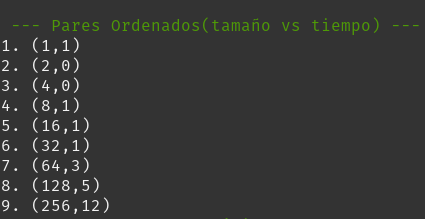
\includegraphics[width=8cm]{Imagenes/Binarios-R-1.png}
                \caption{Resultado en consola de los pares ordenados de (r,t)}
            \end{figure}
            
            \begin{figure}[!h]
            	\centering
            	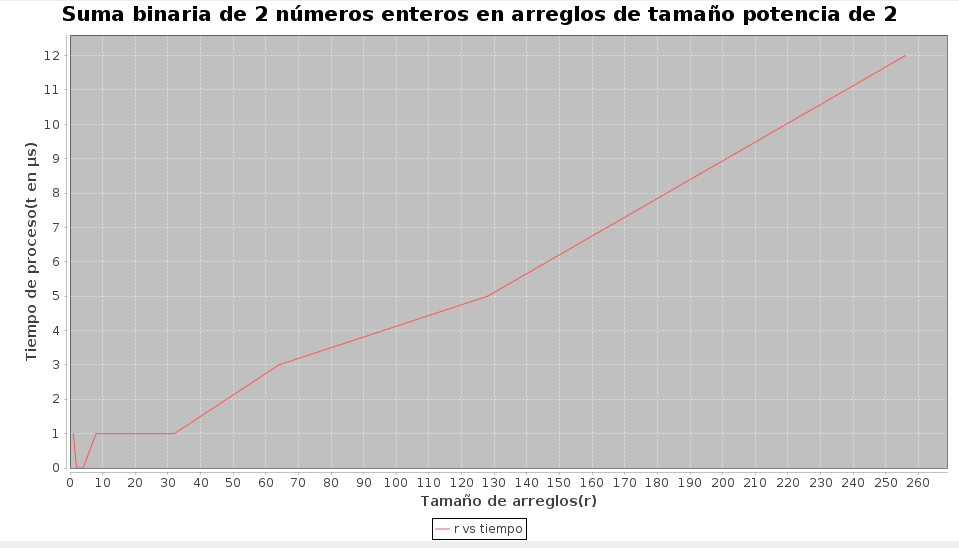
\includegraphics[width=13cm]{Imagenes/Binarios-G-1.png}
                \caption{Gráfica con tendencía a complejidad lineal \textbf{$\theta$(n)}}
            \end{figure}
            
            Se puede observar en la gráficación de los pares ordenados que los primeros valores de \textit{k} tienden a variar de forma caótica por lo que no nos aporta información relevante sobre una aproximación real de la complejidad del algoritmo.\\
            Sin embargo se alcanza a divisar con los últimos valores un patrón que describiría la complejidad del algoritmo como lineal.
            
            \hfill \break
            \hfill \break
                
            \textbf{Gráfica e impresión en consola de los valores de \textit{k}($2^k$) desde 0 hasta 15}
                
            \begin{figure}[!h]
            	\centering
            	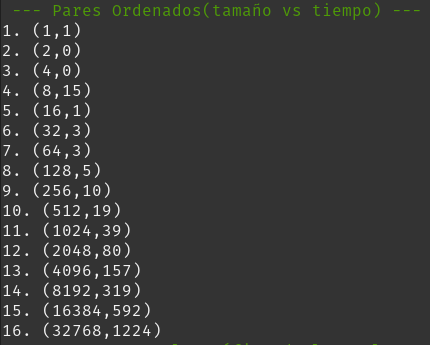
\includegraphics[width=8cm]{Imagenes/Binarios-R-2.png}
                \caption{Resultado en consola de los pares ordenados de (r,t)}
            \end{figure}
            
            \begin{figure}[!h]
            	\centering
            	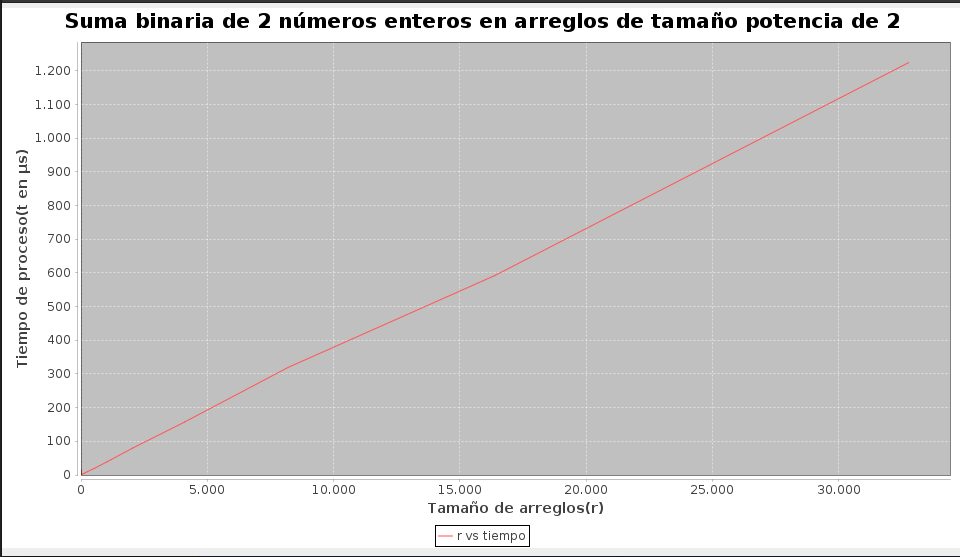
\includegraphics[width=16cm]{Imagenes/Binarios-G-2.png}
                \caption{Gráfica con clara tendencia a complejidad lineal \textbf{$\theta$(n)}}
            \end{figure}
            
            Es claramente observable en esta graficación, una tendencia lineal con muy pocas anormalidades en el trazo de la recta.
            
            
            \hfill \break
            \hfill \break
                
            \textbf{Gráfica e impresión en consola de los valores de \textit{k}($2^k$) desde 0 hasta 20}
                
            \begin{figure}[!h]
            	\centering
            	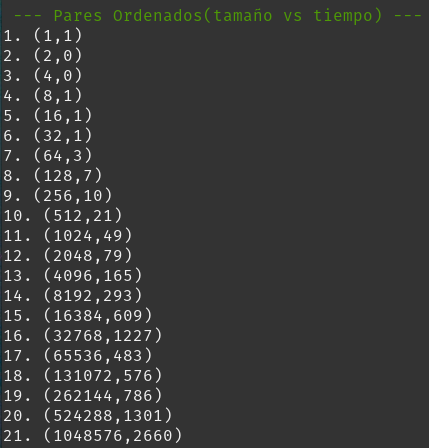
\includegraphics[width=9cm]{Imagenes/Binarios-R-3.png}
                \caption{Resultado en consola de los pares ordenados de (r,t)}
            \end{figure}
            
            \begin{figure}[!h]
            	\centering
            	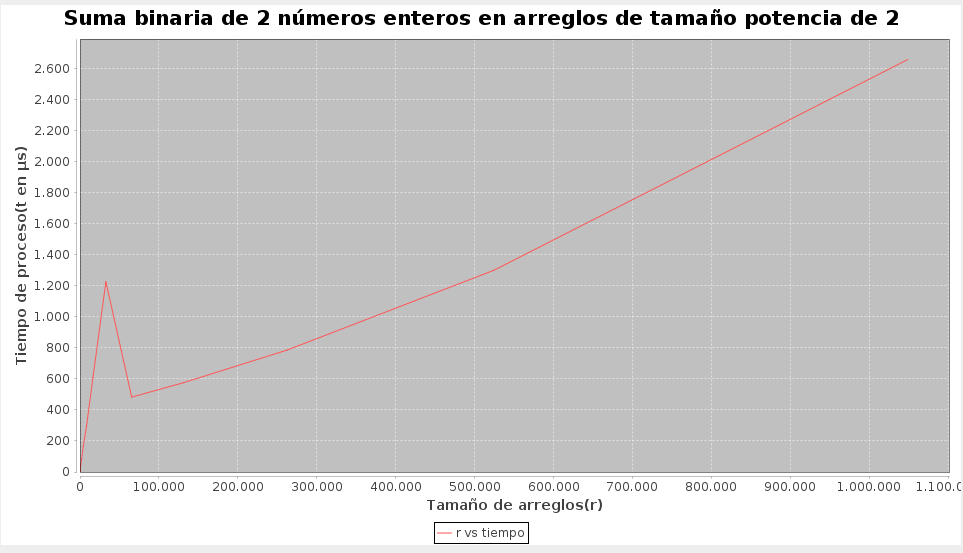
\includegraphics[width=15cm]{Imagenes/Binarios-G-3.png}
                \caption{Gráfica con tendencia a complejidad lineal \textbf{$\theta$(n)} con anormalidad}
            \end{figure}
            
            Para el último caso expuesto en este documento, se tiene una gráfica que toma valores de hasta $2^{20}$ en el eje de las abscisas. Es evidente la anormalidad surgida en el par ordenado \textit{16}, que sin embargo no marca un punto de inflexión o cambio de la tendencia en la que crecen los demás pares, de los que no es necesario decir que crecen linealmente.
            
            \begin{figure}[h]
            	\centering
            	\includegraphics[width=18cm]{Imagenes/Binarios-G-4.png}
                \caption{Gráfica resultante de valor \textit{k} = 27}
            \end{figure}
            
            \end{center}
            
        \subsubsection*{Análisis Asintótico}
        
        Como pudo verse en las gráficas de la sección anterior, el crecimiento descrito por el tiempo de ejecución para diferentes entradas al algoritmo de la suma binaria, muestran una clara similitud con una ecuación que la describe con un crecimiento lineal.\\
        
        Derivado de la misma estructura del algoritmo, identificamos que no existe un mejor o peor caso, por lo que las representaciones mostradas pertenecen a un caso promedio de ejecución del algoritmo. \\
        
        Basándonos en los puntos generados de la monitorización del desempeño con el mayor número de valores, se propone una ecuación:
        $$f(n)=\frac{306}{8191}n $$
        
        Obtenida al usar la ecucación de \textit{recta-pendiente} $y=mx+c$, y la pendiente se calculo con el primer par ordenado $(1,1)$ y el último $(32765,1225)$. Aplicando la ecuación $m=\frac{y_2-y_1}{x_2-x_1}$, el valor es $m=\frac{306}{8191}$
         Bajo la premisa de proponer una función \textit{g(n)} tal que $Suma \in O(g(n)$ y la \textit{g(n)} sea mínima, se propone una de las rectas familias de f(n), a la cual se le suma una constante y que mantenga todos los puntos que exceden a la recta \textit{f(n)} por debajo de esta.
        
        El cálculo exacto de la constante \textit{c}, se encontró al calcular la distancia del punto externo más lejano a la \textit{f(n)}, y se identificó el par ordenado \textit{(4096,165)}. Se utiliza la ecuación para medir la distancia desde la recta a un punto que no este sobre esta:
        $$
            D=|\frac{Ax_1+By_1+c}{\sqrt{A^2+B^2}}|=|\frac{(306)(4096)-(8191)(165)+0}{\sqrt{(306)^2+(-8191)^2}}|\aprox 12
        $$
        
        De esta forma podemos concluir que \textit{c}(Curva color rojo) puede tomar los valores de:$c\geq 12$. Con la $g(n)=\frac{306n}{8191}+12$ cumple su función como cota superior asintótica para toda \textit{n} mayor que 0.\\
        
        Sin embargo, debido a la naturaleza de su cálculo donde se toma un punto exacto de una corrida, y puede haber otro punto en otra corrida que exceda esta \textit{g(n)}. Se propone otra cota que contempla los mas de los puntos y no es demasiado superior a la \textit{f(n)}. Esta \textit{g(n)}(Curva color azul) es $g(n)=\frac{x}{10}$, cumplirá para todos los casos con \textit{n>8}, obteniendo esta limitación no de la curva \textit{f(n)} propuesta, pero de los pares ordenados que muestran puntos con n<8, exterior a la \textit{g(n)}.
        
        
        \begin{landscape}
        Por lo tanto:
            $$g_1(n)=\frac{306n}{8191}+12$$
            $$g_2(n)\frac{x}{10}$$
            $$f(n)=\frac{306n}{8191} \in O(g_1(n)) \in O(g_2(n))$$
            \hfill \break
            \hfill \break
            \hfill \break
            \begin{figure}[!h]
            	\centering
            	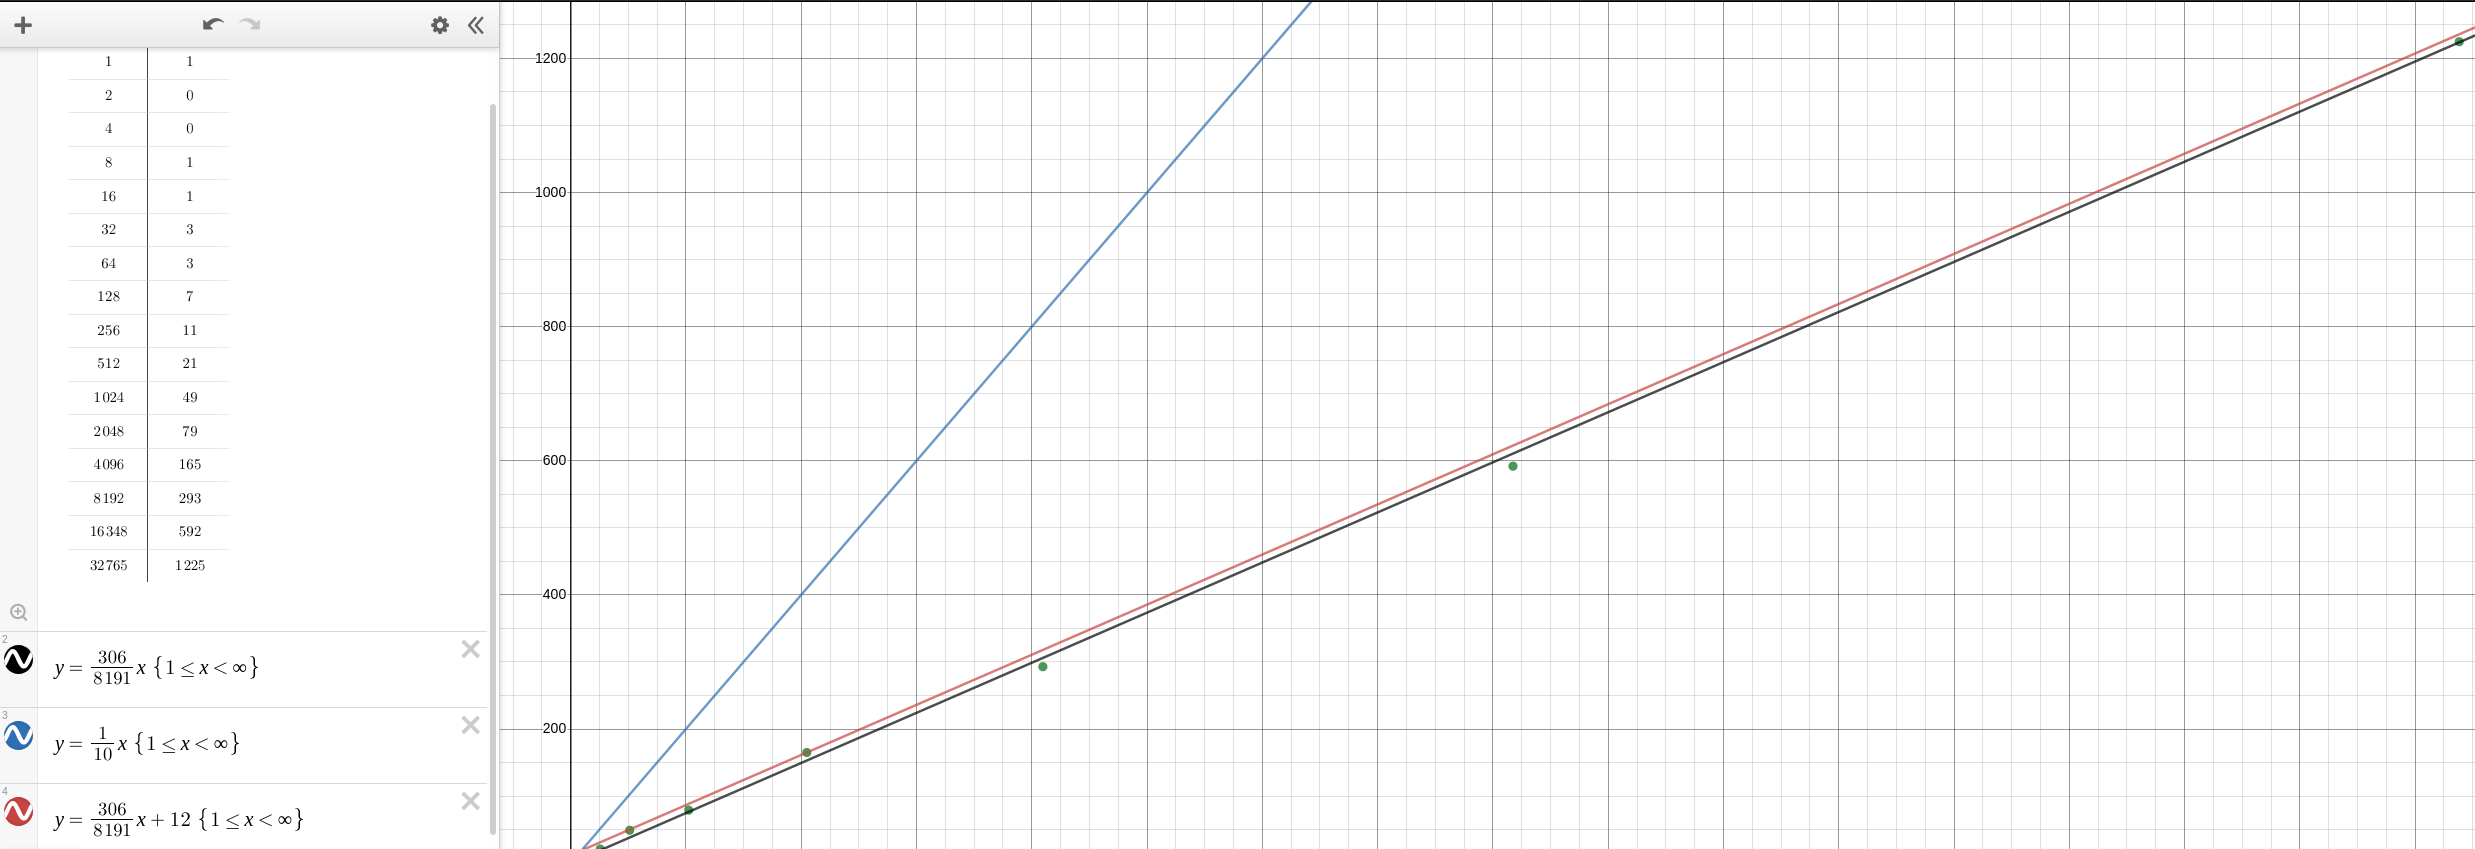
\includegraphics[width=25cm]{Imagenes/Acotaciones-SumaBinaria.png}
                \caption{Dos gráficas propuestas para la acotación de la función propuesta del comportamiento de los pares ordenados}
            \end{figure}
        \end{landscape}
        
       
            
    \subsection*{Algoritmos Euclidiano}
        \subsubsection*{Gráficas de tamaño vs tiempo} 
            Las siguientes gráficas muestra el desempeño del algoritmo con diferentes valores de \textbf{m,n} con respecto al tiempo.\\
            
            En el eje de las abscisas se colocarán los valores de \textbf{m y n}, en el de las ordenadas los valores del tiempo \textbf{t} en $\mu s$. \\
            
            Con la finalidad de mostrar el peor caso de desempeño en este algoritmo se utilizan los valores consecutivos de la sucesión de Fibonacci.
            
            \begin{center}
                \textbf{Gráfica e impresión en consola de los pares ordenados obtenidos de la evaluación de los números en pareja que van desde la primera posición hasta la posición 20 en la sucesión de Fibonacci}
                
            \begin{figure}[!h]
            	\centering
            	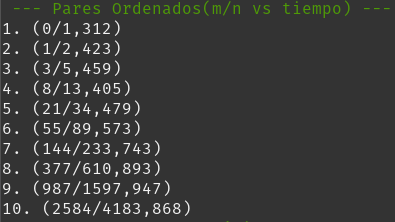
\includegraphics[width=8cm]{Imagenes/MCD-R-2.png}
                \caption{Resultado en consola de los pares ordenados de (m/n,t)}
            \end{figure}
            
            \begin{figure}[!h]
            	\centering
            	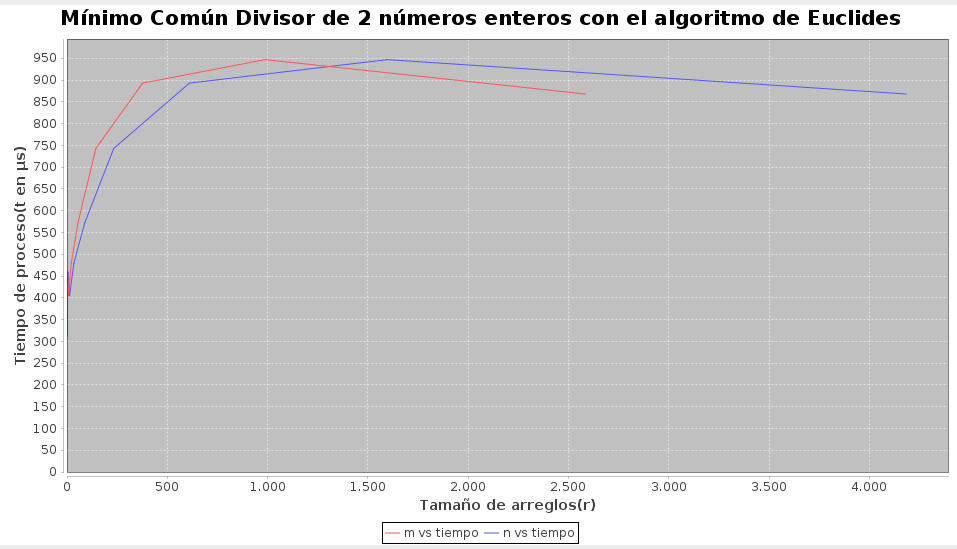
\includegraphics[width=13cm]{Imagenes/MCD-G-2.png}
                \caption{Gráfica con tendencía a complejidad logarítmica \textbf{log(n)}}
            \end{figure}
            
            Se aprecia en la gráfica una curva característica parecida a la de un logaritmo con un desplazamiento en el eje del tiempo.
            
            \hfill \break
            \hfill \break
                
            \textbf{Gráfica e impresión en consola de los pares ordenados obtenidos de la evaluación de los números en pareja que van desde la primera posición hasta la posición 30 en la sucesión de Fibonacci}
                
            \begin{figure}[!h]
            	\centering
            	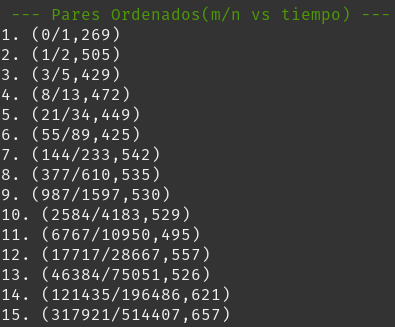
\includegraphics[width=8cm]{Imagenes/MCD-R-3.png}
                \caption{Resultado en consola de los pares ordenados de (m/n,t)}
            \end{figure}
            
            \begin{figure}[!h]
            	\centering
            	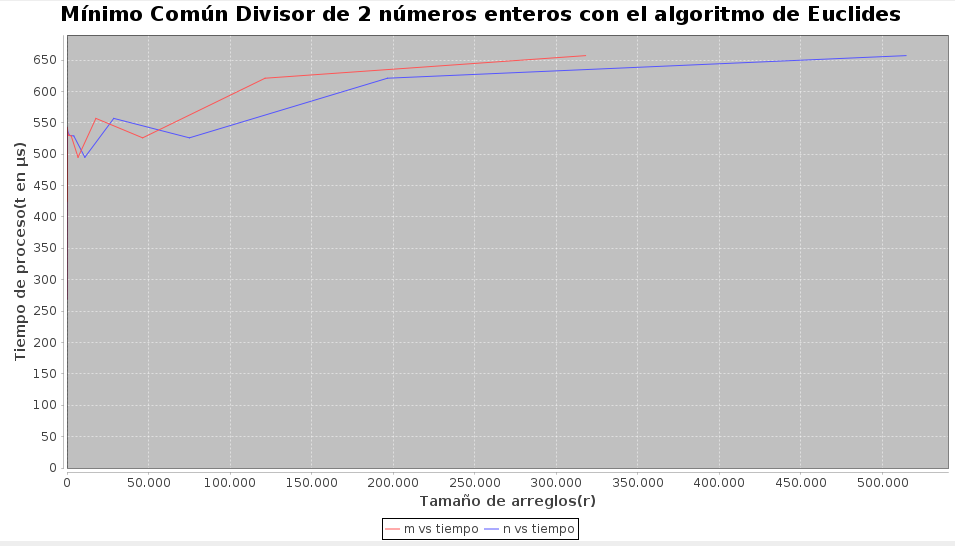
\includegraphics[width=16cm]{Imagenes/MCD-G-3.png}
                \caption{Gráfica con tendencia a complejidad logarítmica \textbf{log(n)}}
            \end{figure}
            
            En perspectiva con la gráfica obtenida anteriormente con un número menor de corridas, se puede apreciar una curvatura menos delicada con una tendencia a un crecimiento muy lento con respecto al eje de las ordenadas.
            
            
            \hfill \break
            \hfill \break
                
            \textbf{Gráfica e impresión en consola de los pares ordenados obtenidos de la evaluación de los números en pareja que van desde la primera posición hasta la posición 40 en la sucesión de Fibonacci}
                
            \begin{figure}[!h]
            	\centering
            	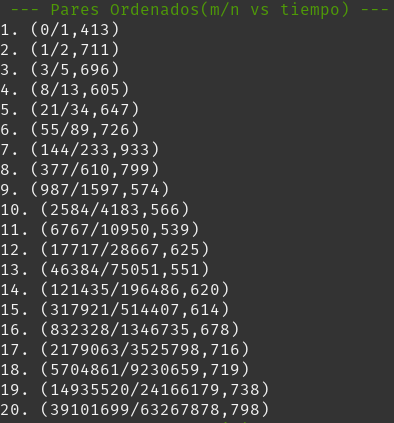
\includegraphics[width=9cm]{Imagenes/MCD-R-4.png}
                \caption{Resultado en consola de los pares ordenados de (m/n,t)}
            \end{figure}
            
            \begin{figure}[!h]
            	\centering
            	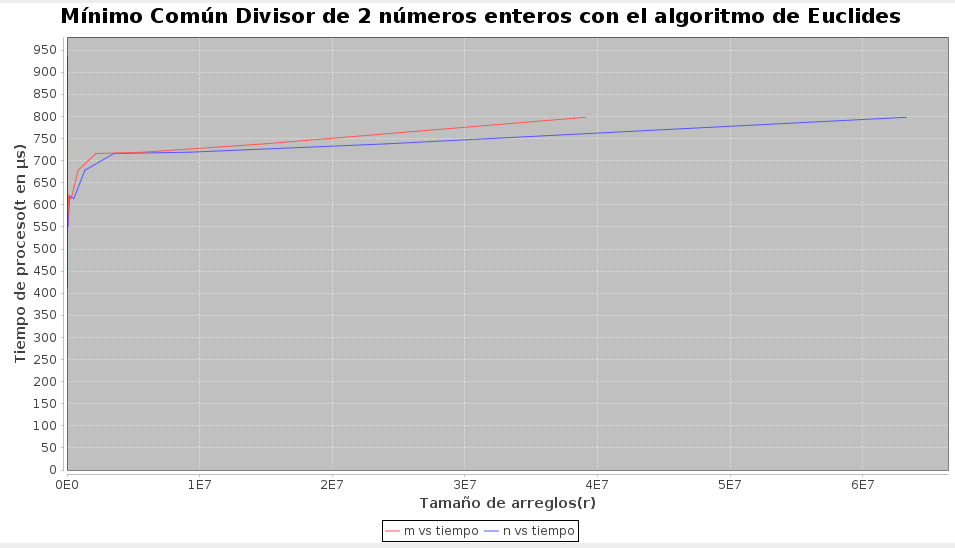
\includegraphics[width=15cm]{Imagenes/MCD-G-4.png}
                \caption{Gráfica con una clara tendencia a una complejidad \textbf{log(n)}}
            \end{figure}
            
            Para el último caso expuesto en este documento, se tiene una gráfica que toma los primeros 40 valores generados de la sucesión de Fibonacci. En esta gŕafica es ahora completamente claro un comportamiento de crecimiento rápido en el eje de las abscisas y en su contraparte, un crecimiento sumamente lento en el de las ordenadas. Esta evidencia nos permite afirmar que el algoritmo tendrá una complejidad en su peor caso de entrada de forma logarítmica \textbf{O(n)}.
            \end{center}
            Como pudo verse en las gráficas de la sección anterior, el crecimiento descrito por el tiempo de ejecución para diferentes entradas al algoritmo de la suma binaria, muestran una clara similitud con una ecuación que la describe con un crecimiento lineal.\\
            
        \begin{landscape}
        \subsubsection*{Análisis Asintótico}
            En comparación con el algoritmo empleado para la suma binaria, este algoritmo si cuenta con un peor caso, y este se muestra en las gráficas anteriores, donde se ingresan parejas de números que son consecutivos en la  suseción de Fibonacci.
            
            Basándonos en los puntos generados de la monitorización del desempeño con el mayor número de valores, se propone una ecuación que necesitará de una constante que la traslade de manera positiva en el eje de las ordenadas:
            $$f(n)=log(n)+800 $$
            
            Estas curva propuesta para la \textit{f(n)}, al no ser una propuesta completamente precisa, ya mantiene los puntos generados por el programa, debajo de la curva. De esta manera ya cumple con la función de cota superior asintótica, sin embargo, para efectos visuales de la captura, se propone otra ecuación, la cual bien hubiera podido tomar un valor con constante \textit{c} en la ecuación $g(n)=clog(n)+800$, de $1 < c <  \infty$. Por simplicidad y practícidad se propone $g(n)=2log(n)+800$, que por lo anterior explicado ya contiene a todos los posibles casos de ejecución por debajo de los límites que marca.
            
            Por lo tanto:
            $$g(n)=2log(n)+800$$
            $$f(n)=log(n)+800 \in O(g(n)$$
            
            
                \begin{figure}[!h]
                	\centering
                	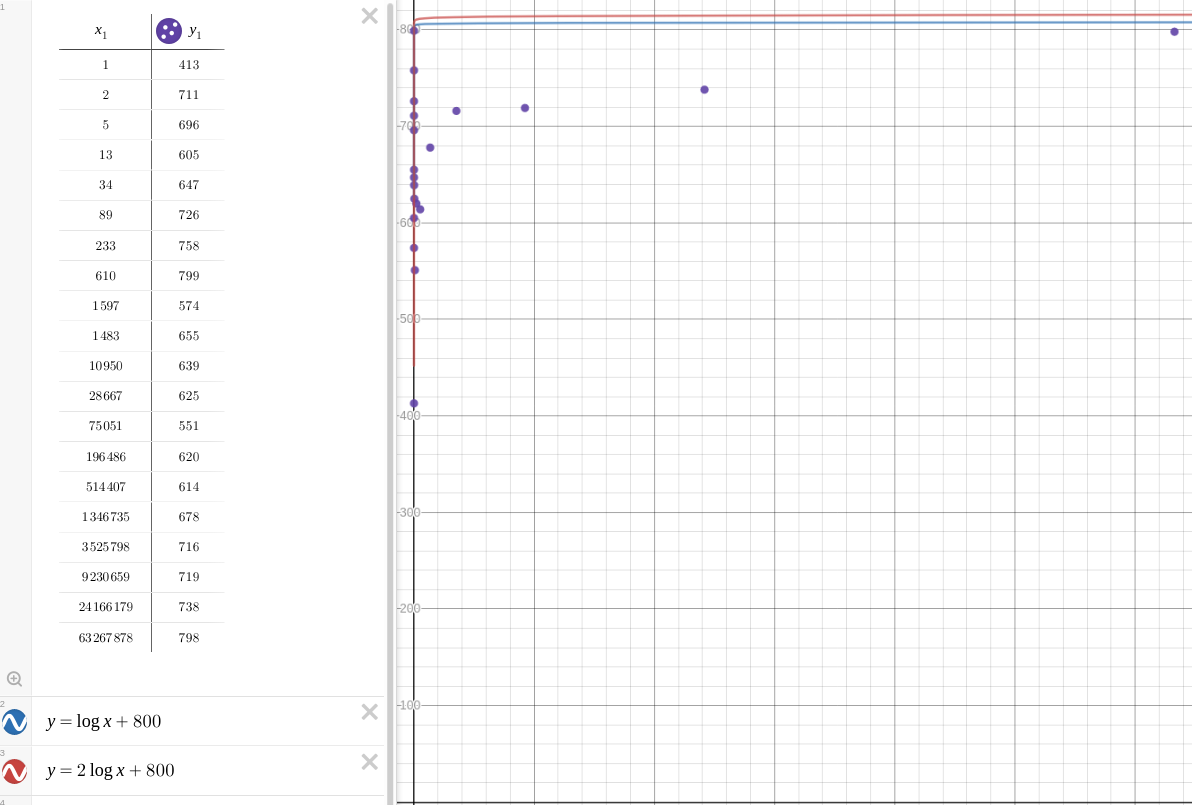
\includegraphics[width=15cm]{Imagenes/Acotacion-Euclides.png}
                    \caption{Curva propuesta para la acotación de la \textit{f(n)} propuesta del comportamiento de los pares ordenados}
                \end{figure}
            \end{landscape}
        
\newpage
\vspace*{3\baselineskip}
\section*{Conclusiones}
    \begin{tabular}{l l}
        \multirow{3}{*}{
\includegraphics[width=1.5cm]{Imagenes/imanol.jpg}} &  \\
        & \textbf{Rivero Ronquillo Omar Imanol}
    \end{tabular}
    \vspace*{3\baselineskip}
    
    Al inicio del diseño cuando nos encontrabamos explorando las posibilidades de implementación del algoritmo de la suma binaria, el primer planteamiento involucraba la utilización de 4 if's para rellenar el arreglo de salida, sin embargo, encontramos m\'as conveniente utilizar el algoritmo que habíamos visto en clases de diseño digital, reduciendo en gran medida la cantidad de código del algoritmo y posiblemente la complejidad del mismo. Posteriormente, nos trajo algunas complicaciones la forma de pasar los parametros a la función y esta hiciera las operaciones de forma autom\'atica sin tener que ingresar las cadenas inmensas para efectuar las sumas, al final utilizamos un random para generar los numeros y un archivo externo para indicar el tamaño que alcanzaria la potencia k. A la hora de la comprobación experimental, notamos que no había un peor caso para el algoritmo.
    
    En el caso del algoritmo de Euclides, se utiliz\'o el algoritmo proporcionado por el profesor. Y utilizamos la misma idea de considerar los valores externos para operar dentro de la funci\'on. El peor caso que comprobamos de forma experimental, fue cuando ingresabamos numero que son consecutivos en la sucesión de Fibonacci.
    
    En conclusión, me pareci\'o realmente interesante explorar la complejidad algoritmica de forma experimental, cosiderando todos los datos que nos fueron arrojados gracias a la forma en la que fue implementada la problematica en nuestro c\'odigo.
    \hfill \break
    \hfill \break
    
    \begin{tabular}{l l}
        \multirow{3}{*}{
\includegraphics[width=1.5cm]{Imagenes/lalo.jpg}}  &  \\
        & \textbf{Valle Mart\'inez Luis Eduardo} \\
        & \\
    \end{tabular}
    
    \vspace*{3\baselineskip}
    La realización de la práctica nos permitió aplicar en un contexto real, las definiciones utilizadas para analizar la complejidad de un algoritmo.
    
    Durante la elaboración de la práctica me enfrenté a algunos problemas derivado principalmente, del desuso de mi parte del lenguaje Java por ya algunos meses. 
    Unido ha esto, existió al principio una confusión con el primer algoritmo y se generaron más métodos que realizaban tareas inecesarias, como la conversión de un número de entrada a cadena binaria. Tiempo más tarde se corrigieron y eliminaron estas funciones, tomando solo en cuenta las cantidades potencias que darían tamaño a los arreglos binarios, y el llenado del arreglo fue una simple función con random.A excepción de esto no hubo mayor complicación en la codificación.
    
    Ya durante la ejecución, la primera vez que las funciones eran llamadas tardaban una cantidad de tiempo anormalmente grande, en comparación de las siguientes ejecuciones, y esto sin se dependientes del valor de entrada. Para evitar esto, se realizó dentro del código, una llamada a las funciones por primera vez, sin contabilizarlas en el registro de pares ordenados. Mostrándo un patrón consistente con los valores esperados de cada entrada.
    
    Otra anomalía que no fue arreglada, se presentó en la graficación de los resultados del primer algoritmo con un conjunto de más de 15 valores y menor a 20, mostrando un pico extraño que desentonaba con la tendencia de comportamiento.
    
    Las gráficas mostradas si tuvieron un resultado aproximado a los valores que esperabamos del desempeño de cada algoritmo.
    
    Finalmente, es posible mejorar el segundo algoritmo mediante el uso de memoización, al igual que en la implementación de algunos algoritmos que genera el valor de la n posición en la sucesión de Fibonacci. Sin embargo esta aproximación mostraría su mejor optimización(con respecto a los recursos y tiempo de procesamiento) cuando la entrada son, precisamente, números pertenecientes a la sucesión de Fibonacci.
\newpage

\begin{thebibliography}{X}
    \bibitem{clase2}Luna,B.[Benjamín Luna].(2020, Septiembre, 29). CLASE 2 - ANÁLISIS DE ALGORITMOS[Archivo de video]. Recuperado de https://www.youtube.com/watch?v=tqzxCTHfv7g.
    \bibitem{clase3}Luna,B.[Benjamín Luna].(2020, Septiembre, 30). CLASE 3 - ANÁLISIS DE ALGORITMOS[Archivo de video]. Recuperado de https://www.youtube.com/watch?v=ojiIVGUU-vI.
   \bibitem{articulo1}Cormen,T., y Balkcom,D.,(2017). Notación $\theta$ grande (Big-$\theta$). Khan Academy. Recuperado de https://es.khanacademy.org/computing/computer-science/algorithms/asymptotic-notation/a/big-big-theta-notation?modal=1.
   \bibitem{articulo2}Cormen,T., y Balkcom,D.,(2017). Notación O grande (Big-O). Khan Academy. Recuperado de https://es.khanacademy.org/computing/computer-science/algorithms/asymptotic-notation/a/big-o-notation?modal=1.
   \bibitem{articulo3}Cormen,T., y Balkcom,D.,(2017). Notación Omega grande (Big-$\Omega$). Khan Academy. Recuperado de https://es.khanacademy.org/computing/computer-science/algorithms/asymptotic-notation/a/big-big-omega-notation?modal=1. 
\end{thebibliography}
\end{document}
